\documentclass[12pt]{article}
\usepackage[top=1in, bottom=1in, left=1in, right=1in]{geometry}

\usepackage{setspace}
\onehalfspacing

\newif\ifeqns
\eqnstrue

\usepackage[hang,flushmargin]{footmisc} 
% 'hang' flushes the footnote marker to the left,  'flushmargin'  flushes the text as well.

\def\baselinestretch{1}
\setlength{\parindent}{0mm} \setlength{\parskip}{0.8em}

\newlength{\up}
\setlength{\up}{-4mm}

\newlength{\hup}
\setlength{\hup}{-2mm}

\usepackage{amssymb}
%% The amsthm package provides extended theorem environments
\usepackage{amsthm}
\usepackage{epsfig}
\usepackage{times}
\renewcommand{\ttdefault}{cmtt}
\usepackage{amsmath}
\usepackage{graphicx} % for graphics files

% Draw figures yourself
\usepackage{tikz} 

% The float package HAS to load before hyperref
\usepackage{float} % for psuedocode formatting
\usepackage{xspace}

% from Denovo Methods Manual
\usepackage{mathrsfs}
\usepackage[mathcal]{euscript}
\usepackage{color}
\usepackage{array}

\usepackage[pdftex]{hyperref}
\usepackage{cancel}

\newcommand{\nth}{n\ensuremath{^{\text{th}}} }
\newcommand{\ve}[1]{\ensuremath{\mathbf{#1}}}
\newcommand{\Macro}{\ensuremath{\Sigma}}
\newcommand{\vOmega}{\ensuremath{\hat{\Omega}}}

\begin{document}
\begin{center}
{\bf NE 250, F17 \\
Diffusion Equation \\ September 7, 2017}
\end{center}

\setlength{\unitlength}{1in}
\begin{picture}(6,.1) 
\put(0,0) {\line(1,0){6.25}}         
\end{picture}

%-------------------------------------------------------------
%\section*{Transport Equation}
%
%Largely from Lewis and Miller Chp.\ 1 \cite{Lewis1993} and Duderstadt and Hamilton Chp.\ 4 \cite{Duderstadt1976}. Note: Duderstadt and Martin \cite{Duderstadt1979} is a very good general reference. It goes through all of this same stuff, but from a slightly more generic point of view (since this applies to \underline{any} collection of neutral particles).

\subsection*{Recap}
The balance of neutrons: rate of change - loss = production. We get what we usually call the Boltzmann Equation for neutron transport
%
\begin{align}
\frac{1}{v}\frac{\partial \psi(\vec{r}, E, \vOmega, t)}{\partial t} &+ 
\vOmega \cdot \nabla \psi(\vec{r}, E, \vOmega, t) +
\Sigma_t \psi(\vec{r}, E, \vOmega, t) = \nonumber\\
%
& \int_{4\pi} d\vOmega' \int_0^{\infty} dE' \Sigma_s(E', \vOmega' \rightarrow E, \vOmega) \psi(\vec{r}, E', \vOmega', t)  +\nonumber\\
%
& \frac{\chi(E)}{4\pi} \int_0^{\infty} dE' \nu(E') \Sigma_f(E') \int_{4\pi} d\vOmega' \psi(\vec{r}, E', \vOmega', t) +
s(\vec{r}, E, \vOmega, t) \nonumber
\end{align}

%--------------------------------------------
%--------------------------------------------
%--------------------------------------------
\section*{Diffusion Equation Derivation}

We will now derive the diffusion equation by \textbf{assuming the angular flux depends only weakly on direction}, $\vOmega$. 
%
% Why?
Why derive the diffusion equation from the transport equation?
\begin{itemize}
\item Nuclear reactions and thus interaction rates only depend on the scalar flux, so that's usually all we need.
\item The angular flux lives in 7-D space (3 space, 2 angle, 1 energy, and 1 time) and the diffusion equation reduces this to 5-D space (3 space, 1 energy, and 1 time), so it's much simpler to solve.
\item Much of the nuclear data is complicated as a function of angle, reducing that complexity makes the data much easier to interact with.
\end{itemize}

The diffusion equation is derived by starting with the transport equation and \textbf{integrating over all angles}. We'll use the \underline{one-group} version for simplicity, but this assumption is not needed for the derivation. 

Recall the definition of scalar flux and net current:
\begin{align*}
\phi(\vec{r}, t) &= \int_{4\pi} d\vOmega \:\psi(\vec{r}, \vOmega, t) \\
\vec{J}(\vec{r}, t) &= \int_{4\pi} d\vOmega \:\vOmega \psi(\vec{r}, \vOmega, t)
\end{align*}

%----------------------------
\subsection*{Neutron Continuity Equation}
Now let's do the integration and go through it term by term:
%
\begin{align*}
\int_{4\pi} d\vOmega\: &\biggl[\underbrace{\frac{1}{v}\frac{\partial \psi(\vec{r}, \vOmega, t)}{\partial t}}_{1} + 
\underbrace{\vOmega \cdot \nabla \psi(\vec{r}, \vOmega, t)}_{2} +
\underbrace{\Sigma_t \psi(\vec{r}, \vOmega, t)}_{3} = \nonumber\\
%
&\underbrace{\int_{4\pi} d\vOmega'\: \Sigma_s(\vOmega' \rightarrow \vOmega) \psi(\vec{r}, \vOmega', t)}_{4} 
+ \underbrace{\frac{\nu \Sigma_f}{4\pi} \int_{4\pi} d\vOmega'\: \psi(\vec{r},  \vOmega', t)}_{5}
+ \underbrace{s(\vec{r}, \vOmega, t)}_{6}\biggr]
\end{align*}
%
This is called the zeroeth order moment w.r.t.\ $\vOmega$. 

\textbf{1.} No approximations
\ifeqns
\begin{equation}
\frac{1}{v}\frac{\partial}{\partial t} \int_{4\pi} d\vOmega \: \psi(\vec{r}, \vOmega, t) = \boxed{\frac{1}{v}\frac{\partial}{\partial t}\phi(\vec{r}, t)}\nonumber
\end{equation}
\else
\vspace*{3em}
\fi

\textbf{3.} No approximations
\ifeqns
\begin{equation}
\Sigma_t \int_{4\pi} d\vOmega \:\psi(\vec{r}, \vOmega, t) = \boxed{\Sigma_t \phi(\vec{r}, t)} \nonumber 
\end{equation}
\else
\vspace*{3em}
\fi

\textbf{5.} No approximations; but we will make use of the identity
\[\int_{4\pi} d\vOmega = \int_0^{\pi} \sin(\theta) d\theta \int_0^{2\pi} d\varphi = 4\pi \]
Thus
\ifeqns
\begin{align*}
\int_{4\pi} d\vOmega\: \frac{\nu \Sigma_f}{4\pi} &\int_{4\pi} d\vOmega' \:\psi(\vec{r},\vOmega', t) = \\
& 4\pi \frac{\nu \Sigma_f}{4\pi} \int_{4\pi} d\vOmega'\: \psi(\vec{r},\vOmega', t) = \boxed{\nu \Sigma_f \phi(\vec{r}, t)}
\end{align*}
\else
\vspace*{5em}
\fi

\textbf{6.} No approximations
\ifeqns
\begin{equation}
\int_{4\pi} d\vOmega \:s(\vec{r}, \vOmega, t) \equiv \boxed{S(\vec{r}, t)} \nonumber
\end{equation}
\else
\vspace*{3em}
\fi

\textbf{4.} Let's further investigate the scattering cross section

Let's interchange the order of integrations over $\vOmega$ and $\vOmega'$:
%
\begin{align*}
\int_{4\pi} d\vOmega\: &\int_{4\pi} d\vOmega'\: \Sigma_s(\vOmega' \rightarrow \vOmega) \psi(\vec{r}, \vOmega', t)\\
%
&= \int_{4\pi} d\vOmega'\: \bigl[ \int_{4\pi} d\vOmega\: \Sigma_s(\vOmega' \rightarrow \vOmega)\bigr] \psi(\vec{r}, \vOmega', t)
\end{align*}

Then we can simplify the scattering term with the assumption (which is often true) that $\Sigma_s(\vOmega' \rightarrow \vOmega)$ is \textbf{azimuthally symmetric}, meaning it only depends on the angle of the scattering cosine $\mu =\vOmega' \cdot \vOmega$.  This implies
\ifeqns
\[\int_{4\pi} d\vOmega \:\Sigma_s(\vOmega' \cdot \vOmega) = 2\pi \int_{-1}^{1} d\mu\: \Sigma_s(\mu) = \Sigma_s\]
\else
\vspace*{3em}
\fi

And therefore:
%
\ifeqns
\begin{align*}
\text{scattering integral }&= \Sigma_s \int_{4\pi} d\vOmega'\: \psi(\vec{r}, \vOmega', t) \\
%
&= \boxed{\Sigma_s \phi(\vec{r}, t)}
\end{align*}
\else
\vspace*{4em}
\fi

\textbf{2.} Finally, we get to the trouble term: streaming
%
\ifeqns
\[\int_{4\pi} d\vOmega \:\vOmega \cdot \nabla \psi(\vec{r}, \vOmega, t) = \nabla \cdot \int_{4\pi} d\vOmega \:\vOmega \psi(\vec{r}, \vOmega, t) = \nabla \cdot \vec{J}(\vec{r}, t)\:. \]
\else
\vspace*{3em}
\fi

\vspace*{2em}
When we put all of the terms together we get the \textbf{neutron continuity equation}. You can see that we have 1 equation, but 2 unknowns (technically 3 equations and 4 unknowns b/c $\vec{J}$ has 3 spatial components):
\begin{equation}
\frac{1}{v}\frac{\partial}{\partial t}\phi(\vec{r}, t) + 
\nabla \cdot \vec{J}(\vec{r}, t) + 
\Sigma_t \phi(\vec{r}, t) =
\Sigma_s \phi(\vec{r}, t) +
\nu \Sigma_f \phi(\vec{r}, t) +
S(\vec{r}, t)\:.
\label{eq:neutroncont}
\end{equation}

We at least have a relationship between $\phi$ and $\vec{J}$.

%-------------------------------------------
\subsection*{First Angular Moment}

The next step is to take the first angular moment of the transport equation to try to develop additional relationships that we can use to solve for $\phi$. Thus, we multiply the one-group TE by $\vOmega$ and integrate over angle (with the zeroth moment, which is what we took to get the continuity equation, we didn't do the multiplication). 

NOTE: at this point I'm dropping the fission term for simplicity (the extension is straightforward). We will assume any fission neutrons are included in our source term, $S$. 

% Identities
We will use the following identities in this part of the derivation:
\begin{align*} 
\int_{4\pi} d\vOmega \:\vOmega &= 0 \qquad \text{because }\vOmega\text{ is an odd function} \\
%
\int_{4\pi} d\vOmega\: \vOmega \vOmega &= \frac{4\pi}{3}\bar{\bar{I}} \qquad \bar{\bar{I}}\text{ is the identity tensor, which means} \\
%
&\int_{4\pi} d\vOmega\: \vOmega_i \vOmega_j = 0 \qquad i \neq j \nonumber \\
&\qquad \qquad = \frac{4\pi}{3} \qquad i = j \nonumber \\
%
\int_{4\pi} d\vOmega \: \vOmega \vOmega \vOmega &= 0 \qquad \\
\end{align*}
%We are going to note that $\vOmega$ is a vector:
%\[\vOmega = \hat{e}_x \underbrace{\sin(\theta) \cos(\varphi)}_{\Omega_x} 
%+ \hat{e}_y \underbrace{\sin(\theta) \sin(\varphi)}_{\vOmega_y}
%+ \hat{e}_z \underbrace{\cos(\theta)}_{\vOmega_z} \]
%
%We will multiply the TE by each component separately to make things a little easier for ourselves. Looking first at $\Omega_x$ 
Multiplying by $\vOmega$ and dropping dependencies when appropriate:
%
\ifeqns
\begin{align*}
\int_{4\pi} d\vOmega\: \vOmega \frac{1}{v}\frac{\partial \psi}{\partial t} &+ 
\int_{4\pi} d\vOmega\: \vOmega \vOmega \cdot \nabla \psi + 
\int_{4\pi} d\vOmega\: \vOmega \Sigma_t \psi =\nonumber \\
&\int_{4\pi} d\vOmega\: \vOmega \int_{4\pi} d\vOmega'\: \Sigma_s(\vOmega' \cdot \vOmega) \psi(\vec{r}, \vOmega', t) +
\int_{4\pi} d\vOmega\: \vOmega s(\vec{r}, \vOmega, t)\:.
\end{align*}
\else
\vspace*{7em}
\fi

Now we can go through term by term, just like how we did to obtain the continuity equation.

\textbf{1.}
\ifeqns
\begin{equation}
\frac{1}{v}\frac{\partial}{\partial t} \int_{4\pi} d\vOmega\: \vOmega \psi(\vec{r}, \vOmega, t) = \boxed{\frac{1}{v}\frac{\partial \vec{J}}{\partial t}} \nonumber
\end{equation}
\else
\vspace*{3em}\\
\fi
%%%%
\textbf{3.} 
\ifeqns
\begin{equation}
\Sigma_t \int_{4\pi} d\vOmega\: \vOmega \psi(\vec{r}, \vOmega, t) = \boxed{\Sigma_t  \vec{J}(\vec{r}, t)} \nonumber
\end{equation}
\else
\vspace*{3em}\\
\fi
%%%%
\textbf{5.} (was 6)
\ifeqns
\begin{equation}
\int_{4\pi} d\vOmega\: \vOmega s(\vec{r}, \vOmega, t) \equiv \boxed{S_{1}(\vec{r}, t)}  \nonumber
\end{equation}
\else
\vspace*{3em}\\
\fi
This is the definition of the first angular moment of the source term. 

%%%%
%\textbf{4.} 
%First, we're flipping the prime order again inside the integral:
%\[\int_{4\pi} d\vOmega' \int_{4\pi} d\vOmega \Omega_x \Sigma_s(\vOmega' \cdot \vOmega) \psi(\vec{r}, \vOmega, t)\]

%We'll use the fact that $\vOmega$ is a unit vector and thus $\vOmega \cdot \vOmega = 1$. We're going to add this into our equation:
%\[ \int_{4\pi} d\vOmega' \bigl[\int_{4\pi} d\vOmega \Omega_x \vOmega \Sigma_s(\vOmega' \cdot \vOmega) \bigr] \cdot \vOmega \psi(\vec{r}, \vOmega, t) \]
%
%Next, recall that $\Sigma_s(\vOmega' \cdot \vOmega)$ depends only on $\mu_0 = \vOmega' \cdot \vOmega$:
%
%\[ 3 \int_{4\pi} d\vOmega' \bigl[\int_{4\pi} d\vOmega \Omega_x \Omega_x' \Sigma_s(\vOmega' \cdot \vOmega) \bigr] \cdot \Omega_x' \psi(\vec{r}, \vOmega, t) \]

\textbf{4.} For the scattering term we will do some mathematical manipulation. There are several ways to do this, but this one makes the most sense to me (different from Duderstadt and Hamilton).

Expand the scattering cross section in Legendre Polynomials, which are a sequence of orthogonal polynomials:
%
\[P_n(x) = \frac{1}{2^n n!}\frac{d^n}{dx^n} \bigl[\bigl( x^2 -1 \bigr)^n\bigr] \:.\]

Use the polynomials as follows and begin writing out terms of the expansion:
\begin{align*}
&\Sigma_s(\vOmega' \cdot \vOmega) = \sum_{l=0}^{\infty} \frac{2l+1}{4\pi} \Sigma_{sl} P_l(\vOmega' \cdot \vOmega) \\
%
&l=0 \text{ is isotropic; (note } P_0 (\vOmega' \cdot \vOmega) = P_0(\mu) = 1 \text{)}\\
&\qquad \Sigma_s(\vOmega' \cdot \vOmega) \cong \frac{1}{4\pi}\Sigma_{s0} \\
%
&l=1 \text{ is linearly anisotropic; (note } P_1 (\vOmega' \cdot \vOmega) = P(\mu) = \mu \text{)}\\
&\qquad \Sigma_s(\vOmega' \cdot \vOmega) \cong \frac{1}{4\pi}\bigl( \Sigma_{s0} + 3 \mu \Sigma_{s1} \bigr) = \frac{1}{4\pi}\bigl( \Sigma_{s0} + 3 \vOmega' \cdot \vOmega \Sigma_{s1} \bigr)
\end{align*}

We're going to \textbf{assume that scattering is at most linearly anisotropic}, so we will stop expanding here.

Substitute the $l=1$ linearly anisotropic truncation into the equation and use some of our identities:
%
\ifeqns
\begin{align*}
\frac{1}{4\pi} \int_{4\pi}  &d\vOmega
\: \vOmega  \int_{4\pi} d\vOmega'\: \bigl[\Sigma_{s0} + 3\vOmega' \vOmega \Sigma_{s1} \bigr] \psi(\vec{r}, \vOmega', t) = \nonumber\\
%
& \underbrace{\frac{1}{4\pi} \int_{4\pi} d\vOmega \:\vOmega}_{0}  \underbrace{\int_{4\pi} d\vOmega'\:  \Sigma_{s0}\psi(\vec{r}, \vOmega', t)}_{\Sigma_{s0} \phi(\vec{r},t)} +
%
\frac{1}{4\pi} \underbrace{\int_{4\pi} d\vOmega \:\vOmega \vOmega}_{4\pi/3 \bar{\bar{I}}} \underbrace{\int_{4\pi} d\vOmega'\: \vOmega' 3  \Sigma_{s1}\psi(\vec{r}, \vOmega', t)}_{3\Sigma_{s1} \vec{J}(\vec{r},t)} \\
%
&= \boxed{\Sigma_{s1} \vec{J}(\vec{r},t)}
\end{align*}
\else
\vspace*{10em}\\
\fi
%%%%%%%%
\textbf{2.} And once again, the trouble term: streaming
%
\ifeqns
\[\int_{4\pi} d\vOmega \:\vOmega \vOmega \cdot \nabla \psi(\vec{r}, \vOmega, t) = \nabla \cdot \int_{4\pi} d\vOmega \:\vOmega \vOmega \psi(\vec{r}, \vOmega, t) \]
\else
\vspace*{3em}
\fi

\vspace*{2em}
All together this is the \textbf{current continuity equation}:
\ifeqns
\begin{equation}
\frac{1}{v}\frac{\partial \vec{J}}{\partial t} 
+ \nabla \cdot \int_{4\pi} d\vOmega \:\vOmega \vOmega \psi(\vec{r}, \vOmega, t) +
\Sigma_t  \vec{J}(\vec{r}, t) =
\Sigma_{s1} \vec{J}(\vec{r},t)
+ S_{1}(\vec{r}, t) \:.
\label{eq:currentcont}
\end{equation}
\else
\vspace*{3em}
\fi

Now we have 2 moment equations that give us 4 total equations (neutron continuity and 3 tensor equations) and 10 unknowns ($\phi$ = 1, $\vec{J}$ = 3, and the new tensor term = 6). 

Taking higher moments by repeating the multiply by $\vOmega$ and integrating isn't going to help matters.


%-----------------------
%-----------------------
\subsection*{Linearly Anisotropic Approximation}
And finally, \underline{we introduce an approximation about the angular flux} (so far we have only approximated the scattering as linearly anisotropic). We now \textbf{assume that the angular flux is at most linearly anisotropic} as well.

To implement this assumption, the angular flux is expanded in angle and only the first two terms are retained (similar to what we just did with scattering):  
%
\begin{align*}
\psi(\vOmega) &\cong  \frac{1}{4\pi}\bigl( \psi_{0} + 3\vOmega \cdot \vec{\psi_{1}} \bigr) \qquad l=1 \text{; linearly isotropic} \\
%
\psi(\vOmega) &\cong \frac{1}{4\pi}\bigl(\phi(\vec{r}, t) + 3 \vOmega \cdot \vec{J}(\vec{r}, t)\bigr) \:.
\end{align*}
The truncated angular flux expansion is then inserted into the streaming term in the current continuity equation, Eqn.\ \eqref{eq:currentcont}, giving 
%
\ifeqns
\begin{align*}
  \nabla \cdot \frac{1}{4\pi} \int d \vOmega \:\vOmega \vOmega  \bigl(\psi_{0} + 3\vOmega \cdot \vec{\psi_{1}}\bigr) &=  
%
\nabla \cdot \frac{1}{4\pi} \bigl[\int d \vOmega \:\vOmega \vOmega  \psi_{0}
%
+ 3 \underbrace{\int d \vOmega \:\vOmega \vOmega \vOmega \cdot \vec{\psi_{1}}}_{0} \bigr] \nonumber \\
% 
&= \nabla \cdot \frac{1}{4\pi} \frac{4\pi}{3}\bar{\bar{I}} \phi(\vec{r}, t) \\
%
  &= \frac{1}{3} \nabla \phi(\vec{r}, t) \:.
\end{align*}
\else
\vspace*{10em}
\fi

With this approximation, the current continuity equation becomes:
\ifeqns
\begin{equation}
\frac{1}{v}\frac{\partial \vec{J}}{\partial t} 
+ \frac{1}{3} \nabla \phi(\vec{r}, t) +
\Sigma_t  \vec{J}(\vec{r}, t) =
\Sigma_{s1} \vec{J}(\vec{r},t)
+ S_{1}(\vec{r}, t) \nonumber
\end{equation}
\else
\vspace*{3em}\\
\fi
%
Next we'll define:
\begin{align*}
\Sigma_a &\equiv \Sigma_t - \Sigma_{s0} \qquad \text{``absorption" cross section}\\
\Sigma_{tr} &\equiv \Sigma_t - \Sigma_{s1} \qquad \text{``transport" cross section}
\end{align*}

Let's substitute these into our equation set: equations \eqref{eq:neutroncont} and \eqref{eq:currentcont}, neutron and current continuity, respectively:
%
\begin{align*}
\frac{1}{v}\frac{\partial}{\partial t}\phi(\vec{r}, t) + 
\nabla \cdot \vec{J}(\vec{r}, t) + 
\Sigma_a \phi(\vec{r}, t) =
%\nu \Sigma_f \phi(\vec{r}, t) +
S(\vec{r}, t) \\
%
\frac{1}{v}\frac{\partial \vec{J}}{\partial t} 
+ \frac{1}{3} \nabla \phi(\vec{r}, t) +
\Sigma_{tr}  \vec{J}(\vec{r}, t) =
S_{1}(\vec{r}, t) 
\end{align*}
%
These are the $P_1$ equations because they are derived from the 0th and 1st Legendre polynomial expansions of the angular flux. And we now have 4 equations with 4 unknowns!

\subsection*{Fick's Law}
If we also assume \underline{steady state} (or weak temporal dependence) and \underline{an isotropic source} ($S_1 = 0$), the current continuity equation becomes
%
\ifeqns
\begin{align*}
\frac{1}{3} \nabla \phi(\vec{r}) +
\Sigma_{tr}  &\vec{J}(\vec{r}) = 0 \\
&\boxed{\vec{J}(\vec{r}) = -\frac{1}{3\Sigma_{tr}} \nabla \phi(\vec{r}) = -D\nabla \phi(\vec{r}) } \qquad \text{Fick's Law}
\end{align*}
\else
\vspace*{7em}\\
\fi
%
where
\[D = \frac{1}{3\Macro_{tr}} = \frac{1}{3(\Macro_t(\vec{r}) - \Macro_{s1}(\vec{r}))}\] 
is the diffusion coefficient. 

 ---------------------------------------\\
\textbf{Aside:} $\Macro_{s1}  = \int d\vOmega \:\vOmega \Macro_{s}$. When we include the azimuthally symmetric assumption we get $\Macro_{s1} = \bar{\mu}_{0}\Macro_{s}$, where $\bar{\mu}_{0}$ is the average cosine of the scattering angle.

For elastic scattering from stationary nuclei when s-wave scattering is present in the center of mass frame, $\bar{\mu_{0}} = \frac{2}{3A}$, where $A$ is atomic mass number. 

With all of this, $\Sigma_{tr} = \Sigma_t - \bar{\mu}_0 \Sigma_s$.

%While we're dealing with the one group version of this, the derivation is technically only valid in one-speed. The reason is that to simplify common procedure to simplify the energy dependence is to \textbf{neglect the anisotropic contribution to energy transfer in a scattering collision}.
%
% Mathematically this means $\Macro_{s1}(E' \to E) = \Macro_{s1}(E) \delta(E' = E)$, giving $\int dE' \:\Macro_{s1}(\vec{r}, E' \to E)J(\vec{r},E') = \bar{\mu_{0}}\Macro_{s}(\vec{r},E)J(\vec{r},E)$.
 ---------------------------------------

\underline{Punchline:} Fick's Law gives us a clear relationship between current and scalar flux. Now we can write the diffusion equation in terms of only $\phi$!
%
\ifeqns
\begin{equation}
\boxed{\frac{1}{v}\frac{\partial}{\partial t}\phi(\vec{r}, t) 
-\nabla \cdot D\nabla \phi(\vec{r}, t) + 
\Sigma_a \phi(\vec{r}, t) =
\nu \Sigma_f \phi(\vec{r}, t) +
S(\vec{r}, t)} \:. \nonumber
\end{equation}
\else
\vspace*{3em}\\
\fi

This equation \textit{now includes several assumptions} that are \textbf{valid} when the solution is \textbf{not} near
%
\begin{enumerate}
\item  a void, 
\item boundary, 
\item source, 
\item or strong absorber.
\end{enumerate} 
%
While these requirements can be quite restrictive, the diffusion equation has been used frequently for analysis of nuclear systems throughout the history of the nuclear industry.

We can also re-write our angular flux expansion as
\[\psi(\vec{r}, \vOmega, t) \cong \frac{1}{4\pi}\Bigl(\phi(\vec{r}, t)  -\frac{1}{\Sigma_{tr}} \nabla \phi(\vec{r}, t)\Bigr) \:.\]

The physical interpretation of the diffusion process is that the ``flow" of neutrons is driven by a spatial gradient of flux. Or rather, neutrons diffuse from high to low concentration areas. You can see the driving function in Fick's Law: 
%
\begin{itemize}
\item Equilibrium is at any location where $\vec{J} = 0$; there are an equal number of neutrons crossing the interface in both directions.
\item When we're not in equilibrium, more neutrons will be scattered from the side with larger $\phi$ to the side with lower $\phi$. Hence the net migration is opposed to the gradient (matching the negative sign). 
\end{itemize}
 

%-----------------------
%-----------------------
\subsection*{Initial and Boundary Conditions}

We now need one initial condition and two boundary conditions. We will also use some other information.

\underline{Mean free path} is the mean distance from the last collision.
\ifeqns
\[\lambda_{t} = \frac{1}{\Sigma_t} \qquad \lambda_{tr} = \frac{1}{\Sigma_{tr}}\]
\else
\vspace*{3em}\\
\fi
%
If scattering is 
\begin{itemize}
\item isotropic, then $\bar{\mu}_0 = 0$ and $\lambda_{tr} = \lambda_{t}$
\item forward peaked, then $\bar{\mu}_0 > 0$ and $\lambda_{tr} > \lambda_{t}$
\end{itemize}	

\textbf{Initial conditions} are pretty easy:
\[\phi(\vec{r}, 0) = \phi_0(\vec{r}) \qquad \forall \vec{r} \in V \:.\]

\textbf{Basic requirements}: the flux must
\begin{itemize}
\item be real and non-negative: $0 \leq \phi$
\item and bounded: $\phi < \infty$ except near mathematical approximations (the source condition). 
\end{itemize}

\subsubsection*{Interface Conditions}
These are also fairly straightforward. With the transport equation, we require that the angular flux be continuous across interfaces: 
\ifeqns
\[\psi_1(\vec{r}_S, \vOmega, t) = \psi_2(\vec{r}_S,\vOmega, t)\qquad \forall \vOmega\:.\]
\else
\vspace*{3em}\\
\fi
For diffusion, we take the 0th and 1st moments of our TE condition and get two equations rather than one. Now
\ifeqns
\begin{align*}
\phi_1(\vec{r}, t) &= \phi_2(\vec{r}, t) \\
\vec{J}_1(\vec{r}, t) &= \vec{J}_2(\vec{r}, t)
\end{align*}
\else
\vspace*{4em}\\
\fi

\subsubsection*{Vacuum Boundary Condition}
These aren't quite so simple. We start by thinking about a non-reentrant condition for the TE where $\vec{r}_s$ is the outside boundary and $\hat{e}_s$ is the unit normal pointing outward: 
\[\psi(\vec{r}_s, \vOmega, t) = 0 \text{ for } \vOmega \cdot \hat{e}_s < 0 \:,\]
%
which is a mathematical statement that there are no neutrons entering our volume. 

To translate this into a diffusion equation statement, we will use \textit{partial currents}: the number of neutrons crossing either inward ($J_{-}$) or outward ($J_{+}$) across a surface:
\ifeqns
\begin{align*}
J_{-}(\vec{r},t) &= \int_{\vOmega \cdot \hat{e} < 0} d\vOmega \: \vOmega \cdot \hat{e}_s \psi(\vec{r}, \vOmega, t) \\
J_{+}(\vec{r},t) &= \int_{\vOmega \cdot \hat{e} > 0} d\vOmega \: \vOmega \cdot \hat{e}_s \psi(\vec{r}, \vOmega, t)\:.
\end{align*}
\else
\vspace*{6em}\\
\fi
We will also say $\int_{\vOmega \cdot \hat{e} < 0} = \int_{2\pi^{-}}$ and  $\int_{\vOmega \cdot \hat{e} > 0} = \int_{2\pi^{+}}$. 

With this notation we can re-write our boundary condition:
\[J_{-}(\vec{r}_s,t) = \int_{2\pi^{-}} d\vOmega \: \vOmega \cdot \hat{e}_s \psi(\vec{r}_s, \vOmega, t) = 0 \:,\]
note that in diffusion theory
\[\psi(\vec{r}_s, \vOmega, t) \cong \frac{1}{4\pi}\bigl(\phi(\vec{r}_s, t)  -\frac{1}{\Sigma_{tr}} \nabla \phi(\vec{r}_s, t)\bigr)\]
%
and then our partial currents become (note that which of +/- you choose depends on which edge of the problem you are on)
%
\ifeqns
\begin{align*}
J_{-} &= \int_{2\pi^{-}} d\vOmega \: \vOmega \cdot \hat{e}_s \psi(\vec{r}_s, \vOmega, t) =\\
&\cong \frac{1}{4} \phi(\vec{r}_s, t) \mp \frac{D}{2} \hat{e}_s \cdot \nabla \phi(\vec{r}_s, t) = 0\:.
\end{align*} 
\else
\vspace*{6em}\\
\fi
%
For a 1-D slab with a vacuum boundary at $x=x_s$:
%
\begin{align*}
J_{-}(\vec{r}_s, t) = J_{-}(x_s, t) &= \frac{1}{4} \phi(x_s, t) + \frac{D}{2}\frac{d \phi}{dx}\Bigm\lvert_{x_s} = 0 \\
\text{Or } \qquad \frac{1}{\phi(x_s, t)}\frac{d \phi}{dx}\Bigm\lvert_{x_s} &= -\frac{1}{2D}
\end{align*}

This relationship implies that linearly extrapolating the flux beyond the vacuum boundary would lead to a vanishing flux at the point
\[\tilde{x}_s = x_s + 2D = x_s + \frac{2}{3}\lambda_{tr}\:.\]
%
Thus, the vacuum condition $J_{-}(x_s) = 0$ is usually replaced with $\phi(\tilde{x}_s)= 0$. Additionally, computation with more detailed transport theory leads to an \textbf{extrapolation distance} of $0.7104\lambda_{tr} = z_0$ rather than $\frac{2}{3}\lambda_{tr}$. 

DRAW PICTURE
%
\begin{figure}[h!]
\begin{center}
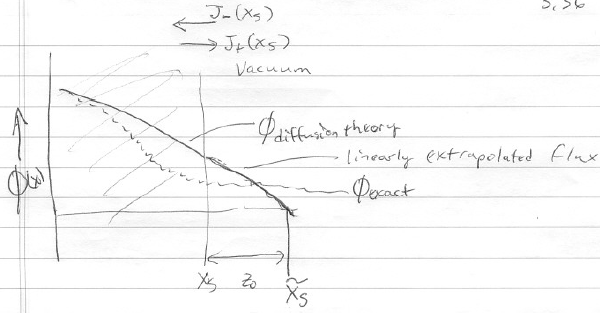
\includegraphics[height=3 in]{../figs/DiffusionBC}
\end{center}
\end{figure}

In reality, though, $\lambda_{tr} \sim 0$ [cm] compared to the size of a reactor core [m]. 


%------------------------------------------
\subsection*{Helmholtz Form}
In steady state, we can write the diffusion equation this way:
%
\ifeqns
\begin{align*}
-\nabla \cdot D\nabla \phi(\vec{r}) + 
\Sigma_a \phi(\vec{r}) &= Q(\vec{r})\:, \\
%
\text{where }\qquad Q(\vec{r}) &=
\nu \Sigma_f \phi(\vec{r}) +
S(\vec{r})\:,
\end{align*}
\else
\vspace*{4em}\\
\fi
%
which can be written as the Helmholtz equation of applied mathematics:
%http://en.wikipedia.org/wiki/Helmholtz_equation
%
\begin{align*}
\nabla^2 \phi(\vec{r}) - \frac{1}{L^2}\phi(\vec{r}) &= \frac{-Q(\vec{r})}{D}\:, \\
\text{where }\qquad L &\equiv \sqrt{\frac{D}{\Sigma_a}}\:.
\end{align*}
%
$L$ is called the neutron diffusion length. This is ``how far a neutron diffuses from a source prior to absorption". 

In the Helmholtz formulation, $\phi$ is amplitude and $\frac{1}{L}$ is wave number. 

This formulation is useful because we know how to solve it. We write
\[\phi(\vec{r}) = \phi_H(\vec{r}) + \phi_P(\vec{r}) \:,\]

For example, we often have:
\[\phi_H(\vec{r}) = A\exp\bigl(-\frac{|\vec{r}|}{L}\bigr) + B\exp\bigl(\frac{|\vec{r}|}{L}\bigr) \:.\]

Going through how to solve this analytically in a variety of circumstances, geometries, etc.\ is another class (NE 150/250). We're going to focus on numerical solution techniques. But first, one more thing.

%------------------------------------------
\subsection*{Criticality Calculations}

We can write our DE in steady state for a nuclear reactor core:
%
\begin{align*}
-\nabla \cdot D\nabla \phi(\vec{r}) + 
\Sigma_a \phi(\vec{r}) &= \nu \Sigma_f \phi(\vec{r})\:, \\
\text{with} \qquad \phi(\tilde{x}_s) &= 0\:.
\end{align*}
%
Unless we have the proper combination of core composition ($\Sigma_a$, $\Sigma_f$, $D$) and geometry ($\vec{r}$ ,$\vec{r}_s$) details, there is \underline{no} general solution. 

To deal with this, we introduce a parameter $k$ into the equation:
%
\ifeqns
\begin{equation}
-\nabla \cdot D\nabla \phi(\vec{r}) + 
\Sigma_a \phi(\vec{r}) = \frac{1}{k}\nu \Sigma_f \phi(\vec{r})\:. \nonumber
\end{equation}
\else
\vspace*{3em}\\
\fi
%
Then, for any value of $k$ we assert that there is always a solution. We use an iterative process to find the condition when $k=1$, called ``critical''.

A reactor is called \textbf{``critical''} if the chain reaction is self-sustaining and time-independent. Another way to think of the addition of $k$ is to assume $\nu$ can be adjusted to obtain a time-independent solution by replacing it with $\frac{\nu}{k}$, where $k$ is the parameter expressing the deviation from critical. 

This substitution changes the transport equation into an \textbf{eigenvalue problem.} A spectrum of eigenvalues can be found, but at \textbf{long times only the non-negative solution corresponding to the largest real eigenvalue will dominate}, and that's $k$. 

$k$ can also be thought of as the asymptotic ratio of the number of neutrons in one generation to the number in the next.

%%--------------------------------------------------------------------
%\bibliographystyle{plain}
%\bibliography{../03-te/te-de} 

\end{document}
